\documentclass{article}

\usepackage{graphicx}
\usepackage{amsmath,amsfonts,amssymb}
\usepackage[colorlinks,bookmarks,bookmarksnumbered,allcolors=blue]{hyperref}
\usepackage[capitalise]{cleveref}
\usepackage[top=0.75in]{geometry}

\begin{document}

\author{Andrew Ning and Judd Mehr}
\title{Leapfrogging Vortices}
\date{}  %May 10, 2019}
\maketitle

Vortex rings are pretty neat.  Read this \href{https://en.wikipedia.org/wiki/Vortex_ring}{wikipedia article} to get an idea of what they are.  They can propel themselves quite far when moving through a quiescent fluid.  See some fun videos of vortex rings formed by \href{https://www.youtube.com/watch?v=VbV98Z0QP-k}{a volcano}, \href{https://www.youtube.com/watch?v=ks3aQhEohTE}{dolphins}, and  \href{https://www.youtube.com/watch?v=72LWr7BU8Ao}{a plate in a pool}.  They can also be dangerous, for example with helicopters that \href{https://youtu.be/wddpsnvu0PM?t=75}{descend too quickly}.

If you're really careful, and put one vortex ring right behind another you can have leapfrogging vortices!  Check out this video of a \href{https://youtu.be/Yydb9Mqg9TY}{real-life visualization} of the phenomenon, as well as a \href{https://youtu.be/0LP-MgrXtIM}{2D simulation}, and a neat \href{https://www.youtube.com/watch?v=SPBMEXX5xBI}{3D simulation}.

First a little background.  A single vortex produces a velocity field as shown in \cref{fig:vortex}.  It's a lot like the flow field you might see in a bathtub drain on in a hurricane.  A vortex causes the flow to spin around it in the tangential direction as given by:
\begin{equation}
V_\theta = \frac{\Gamma}{2 \pi r}
\end{equation}
The variable $\Gamma$ is the strength of the vortex and is also called the \emph{circulation}.  If we increase $\Gamma$ then the induced velocities increase proportionally.  Notice that the strength of the vortex decreases as $1/r$.  Thus, really close to the vortex the induced velocities are high (indicated by the longer arrows) and as we move further away from the vortex its strength approaches zero.  The vortex does not induce any radial velocity ($V_r = 0$).

\begin{figure}[htb]
\centering
\includegraphics[width=3.0in]{vortex}
\caption{A point vortex (in blue) inducing a velocity field (in black) with the equation describing the velocity field to the right.}
\label{fig:vortex}
\end{figure}


With that basic background we can simulate leapfrogging vortices in 2D.  If you picture a toroidal vortex intersecting a 2D plane you will have two vortices (like the left pair shown in \cref{fig:vortices}).  From our understanding of vortices we can see how it is self-propelling.  Consider the left pair of vortices (e.g., one ring vortex).  The top vortex induces a velocity on the bottom vortex towards the right.  Simultaneously, the top vortex induces a velocity on the top vortex to the right.  Thus, it pushes itself forward.  With two vortices next to each other, things become even more interesting.

\begin{figure}[htb]
\centering
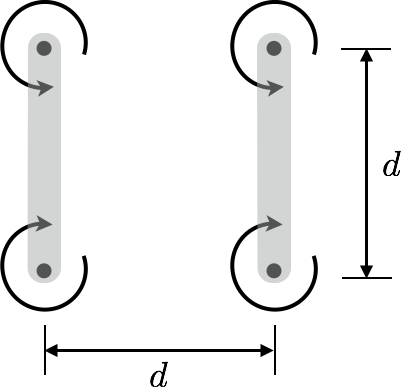
\includegraphics[width=1.5in]{vortices}
\caption{A pair of leapfrogging vortices.}
\label{fig:vortices}
\end{figure}

In this example, make all vortices of equal strength ($\Gamma$).  Each vortex is free to move, and moves with the local fluid velocity.  We will use a basic time stepping method.  Imagine simulating the flight of a ball after it is thrown (we include air resistance so we can't just precompute it using kinematics).  One way to do this is to discretize its motion into small segments of time.  Let's say we have the way to compute the velocity of the ball, if we simulate some small time interval, say a tenth of a second, we could multiply the velocity vector by that time interval and estimate where the ball would have moved at the end of that interval.  We move the ball, recompute the velocity vector, and repeat. This approach is an approximation because the velocity vector really changes continuously and doesn't follow straight lines during time intervals.  However, if we chose a small enough time step the real behavior will be well represented.

Using this procedure you will need to compute the influence of each vortex on every other.  From that induced velocity you can then update the location of all the vortices and repeat.  You need to use a small enough time step to ensure stability.  You may need to try smaller time steps to make sure that your simulation is accurate.

Hint (if you're comfortable with vectors): In vector form, the induced velocity from a vortex is:
\begin{equation}
    \begin{aligned}
        \vec{V} &= \frac{\vec{\Gamma} \times \hat{r}}{2 \pi r}\\
        &= \frac{\vec{\Gamma} \times \vec{r}}{2 \pi r^2}
    \end{aligned}
\end{equation}


\clearpage
\newpage

\subsubsection*{Example Calculations}

In order to help you make sure you're heading in the right direction, we'll do some example calculations for the following case:

\renewcommand{\arraystretch}{1.5}
\begin{tabular}{r | l}
	Parameter & Value \\
	\hline
	$\Gamma$ & $[0,0,1]^\top$ \\
	d & 1.0 \\
	$\Delta t$ & 0.01
\end{tabular}

\noindent where we are going to let the cross-sectional vortices as shown in \cref{fig:vortices} be numbered 1 through 4 starting with the bottom left and moving clockwise.

The following tables show the values for position, P, and velocity, V, (rounded to the nearest 1/1000) at the \textit{beginning} of the first couple time steps for your reference. Note that they are vectors of the form [x,y].

\renewcommand{\arraystretch}{1.5}
\begin{tabular}{r | l | l | l | l }
	Time Step & P1 & P2 & P3 & P4  \\
	\hline
	0  & [0.0,-0.5] & [0.0,0.5] & [1.0,0.5] & [1.0,-0.5]   \\
	1 & [0.002,-0.499] & [0.002,0.499] & [1.002,0.501] & [1.002,-0.501]
\end{tabular}

\bigskip

\renewcommand{\arraystretch}{1.5}
\begin{tabular}{r | l | l | l | l  }
	Time Step & V1 & V2 & V3 & V4 \\
	\hline
	0   & [0,0] & [0,0] & [0,0] & [0,0]  \\
	1 & [0.239, 0.0796] & [0.239, -0.0796] & [0.239, 0.0796] & [0.239, -0.0796]
\end{tabular}

Once you have the pieces working together, you can compare your end results with \cref{fig:vortexpaths}, an example solution for what your vortex ring paths might look like.

\begin{figure}[htb]
	\centering
	\includegraphics[width=\textwidth]{paths.pdf}
	\caption{Paths for the leapfrogging vortex rings using $\Gamma = [0,0,1]^\top$, an initial distance of $d=1.0$, and a time step of $\Delta t =0.01$, over 4000 time steps.}
	\label{fig:vortexpaths}
\end{figure}


\end{document}